\vspace*{-5mm}
\mysection{Runtime View}
In this section we will see some Runtime Views in order to see how the components interact according to specific requests.\par
For the server-side we have taken into consideration the high-level Application Server only, without identifying the specific components of it. We also separate it from the DB, cause they are in 2 different machines.

\mysubsection{EasyLib}
\vspace*{0.5cm}

\mysubsubsection{QR-Code Scan + Book Reservation}
This Runtime View shows the different steps needed to find book information through QR-code scan and reserve it.\par
We have to make an assumption : in the following diagram we reported only the most meaningful calls needed to achieve the goal.\par
So starting from the Main Activity the User has to tap the “QR scan” icon on the bottom NavBar and the EasyLib app will open the “QR Scan Activity”. Thanks to the camera of the smartphone or tablet the QR-image is captured and an identifier is returned. This one is the book identifier and is sent to the server (and so the DB) to get back the information. The “Book Activity” is started and book information are set in the layout.\par
In order to let the user reserve the book, the app gets from the server (and so the DB) a list of libraries where it’s available. They are next passed to the BookActivityAdapter that creates the single items of the recyclerView placed under the book information.
\newpage
\vspace*{0cm}
\begin{figure}[H]
	\centering
	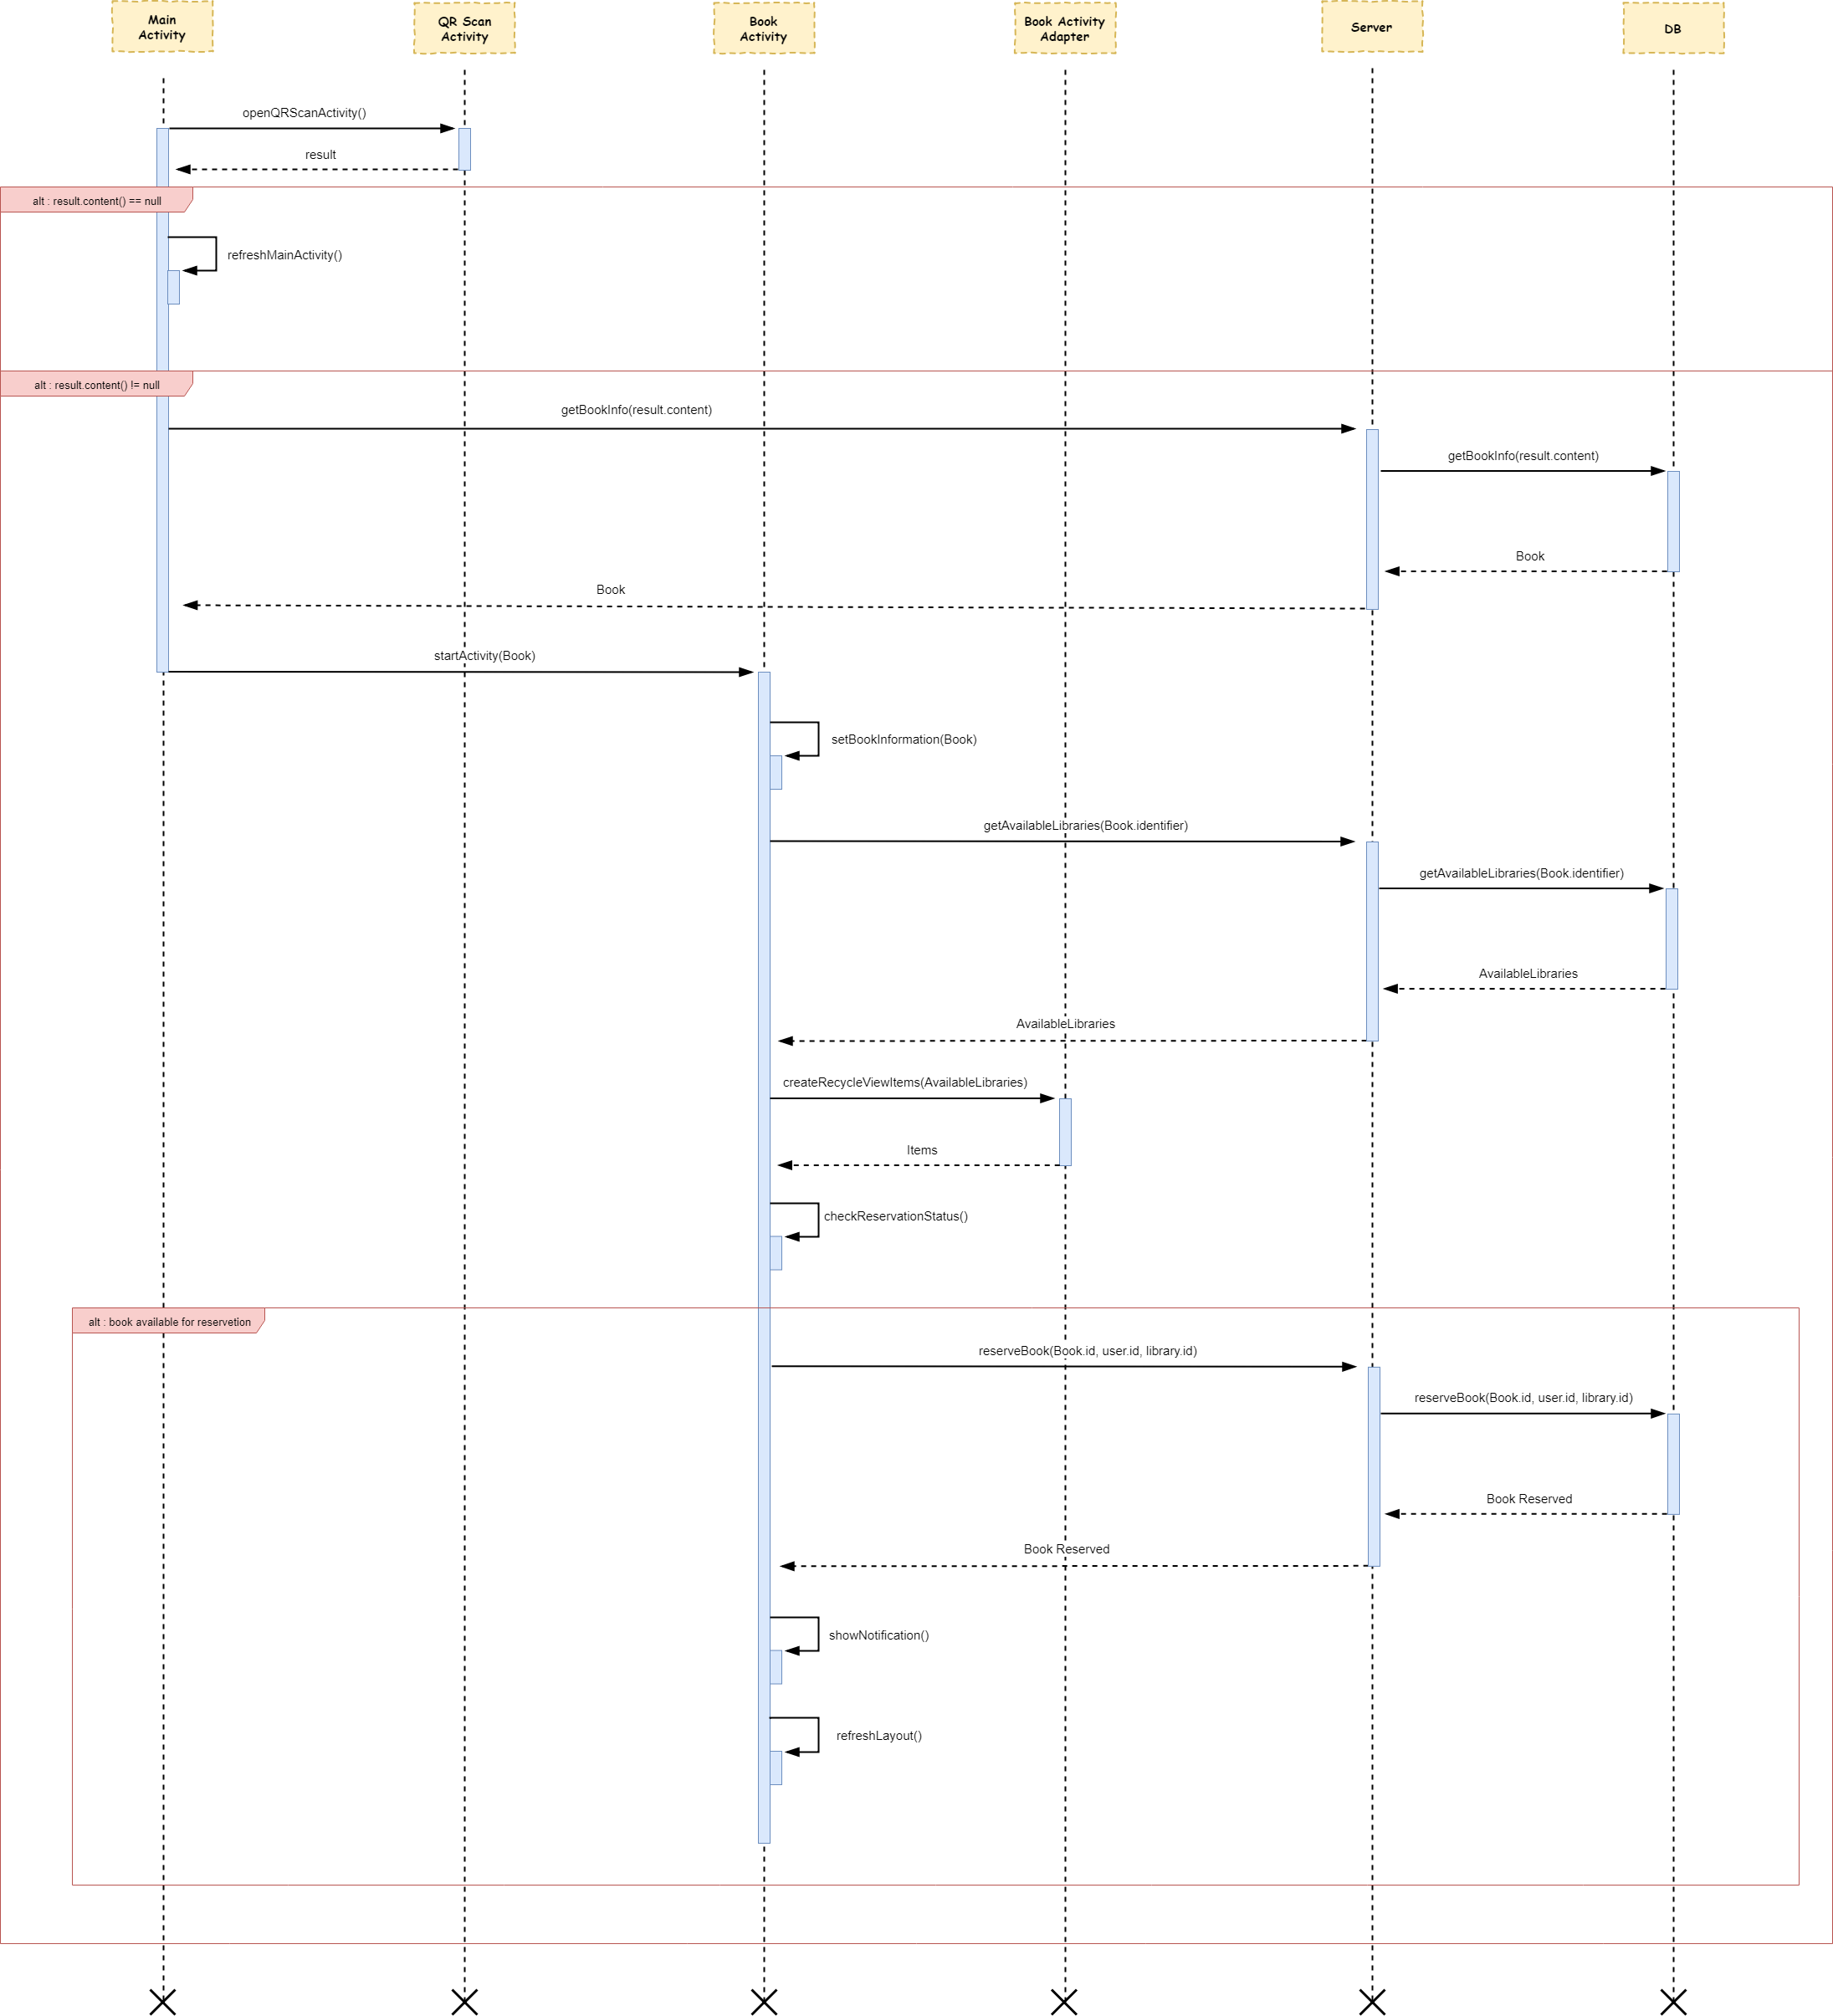
\includegraphics[scale=0.21]{Images/Runtime/user_qrcode_reserve}
	\caption{QR-Code Scan + Book Reservation - Runtime View}
\end{figure}

\newpage
\vspace*{0cm}
\mysubsubsection{Rate Book}
This Runtime View shows the different steps needed to rate a book.
We have to make some assumption :
\begin{itemize}
	\setlength{\leftskip}{0.5cm}
	\item In the following diagram we reported only the most meaningful calls needed to achieve the goal.
	\item The book can be rated only if it was previously reserved and read through EasyLib app.
\end{itemize}
So starting from the Main Activity the User has to tap the “Profile” icon on the bottom NavBar and the EasyLib app will ask the server for User information sending his user identifier. Once data are back, "Main Activity" sets the "Profile Fragment" in the Main Frame.\par
Next the app asks the server for the read books and shows them in the "Read Books Activity" that contains a recyclerView. The user can select the wanted book and open it in the "Book Activity". When it starts the book information, passed with an Intent, are set in the layout and a check is made in order to see if the it's already rated by the user or not. In case it's not, an EditText is showed and the user can fill it with a rate from 0 to 10.
\newpage
\vspace*{0cm}
\begin{figure}[H]
	\centering
	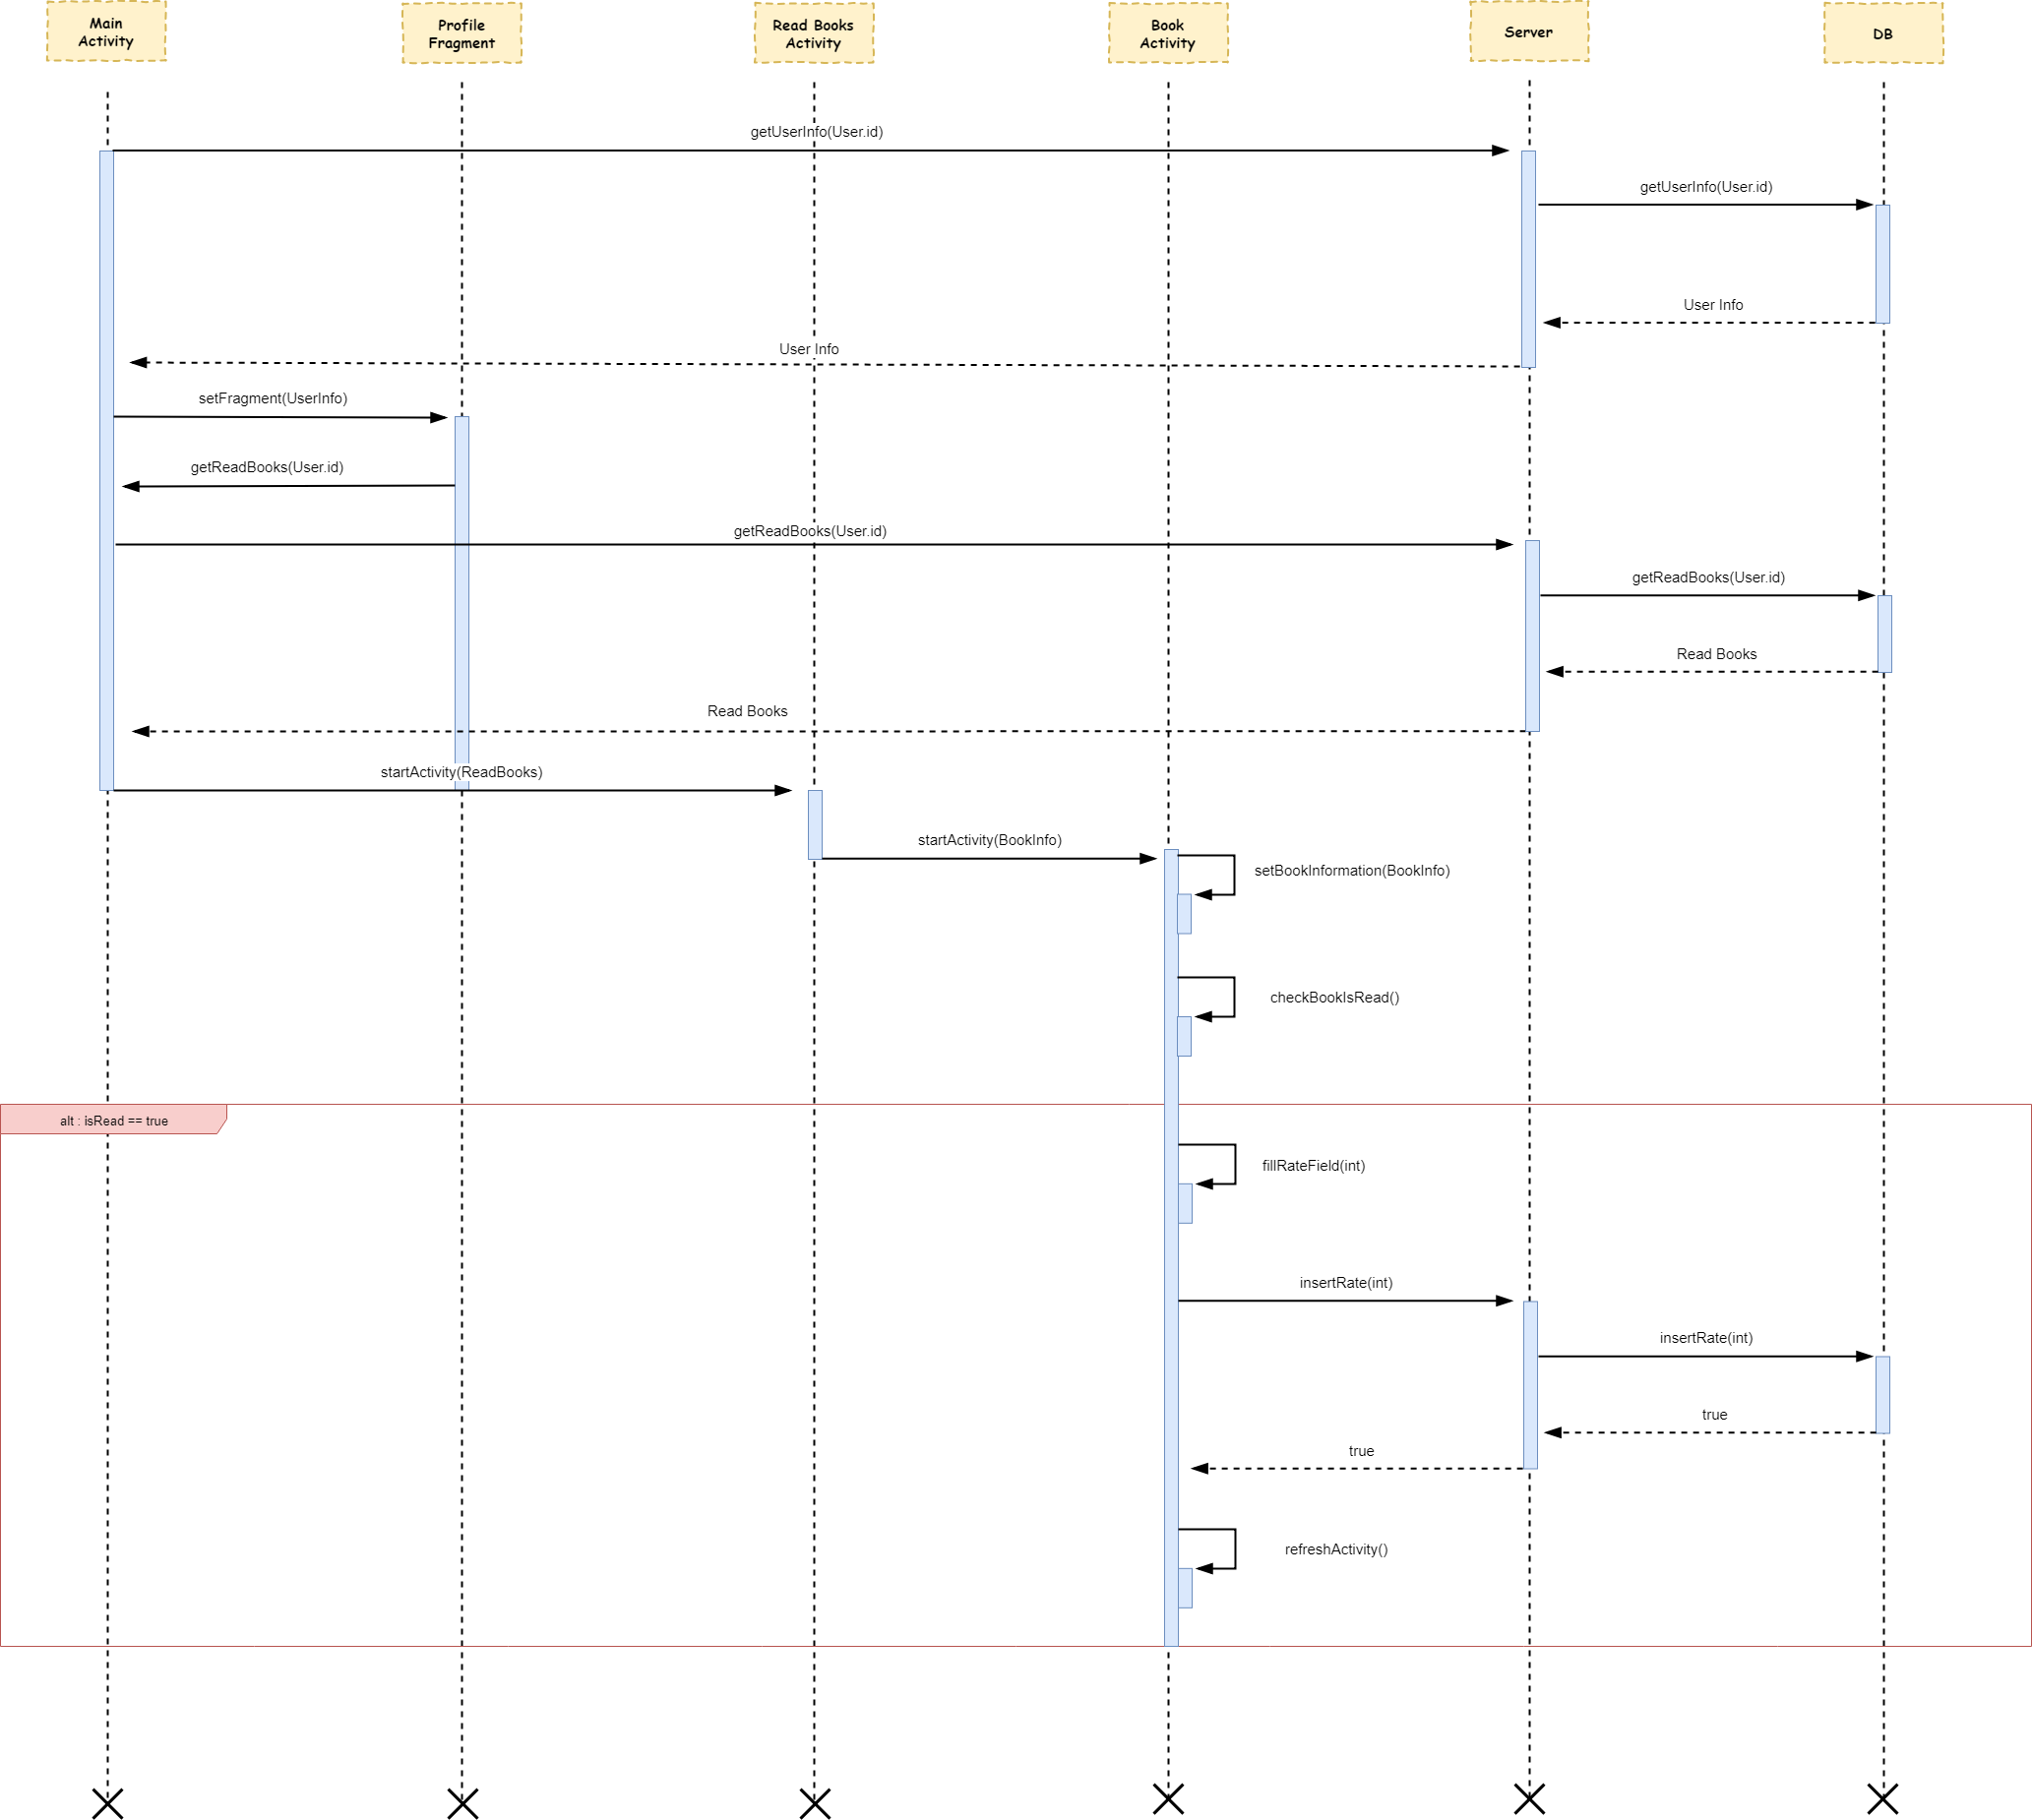
\includegraphics[scale=0.22]{Images/Runtime/rate_book}
	\caption{Rate Book - Runtime View}
\end{figure}

\newpage
\vspace*{0cm}
\mysubsubsection{Event - Reserve Seat}
This Runtime View shows the different steps needed to reserve a seat. \par
We have to make an assumption : in the following diagram we reported only the most meaningful calls needed to achieve the goal. \par
So starting from the Main Activity the User can tap the “All Libraries” button and the EasyLib app will ask the server (and so the DB) to get the list of all of them. On return a new activity is started where thanks to a RecyclerView the list of all the libraries is displayed. \par
The user can next select the Library that he wants and like the libraries list, the information about this one are asked to the server and next displayed in the Book Activity. In this activity are displayed also the “library contents” (news, events and books), so user can select an event and automatically the EventActivity is opened and shown.\par
The app will check if there are available seats and if the user has already joined the event (in the diagram is called “checkEventStatus()”). So if there free seats and the event is not already joined then the “Reserve Seat” button is shown and the User can reserve a seat.
\newpage
\vspace*{0cm}
\begin{figure}[H]
	\centering
	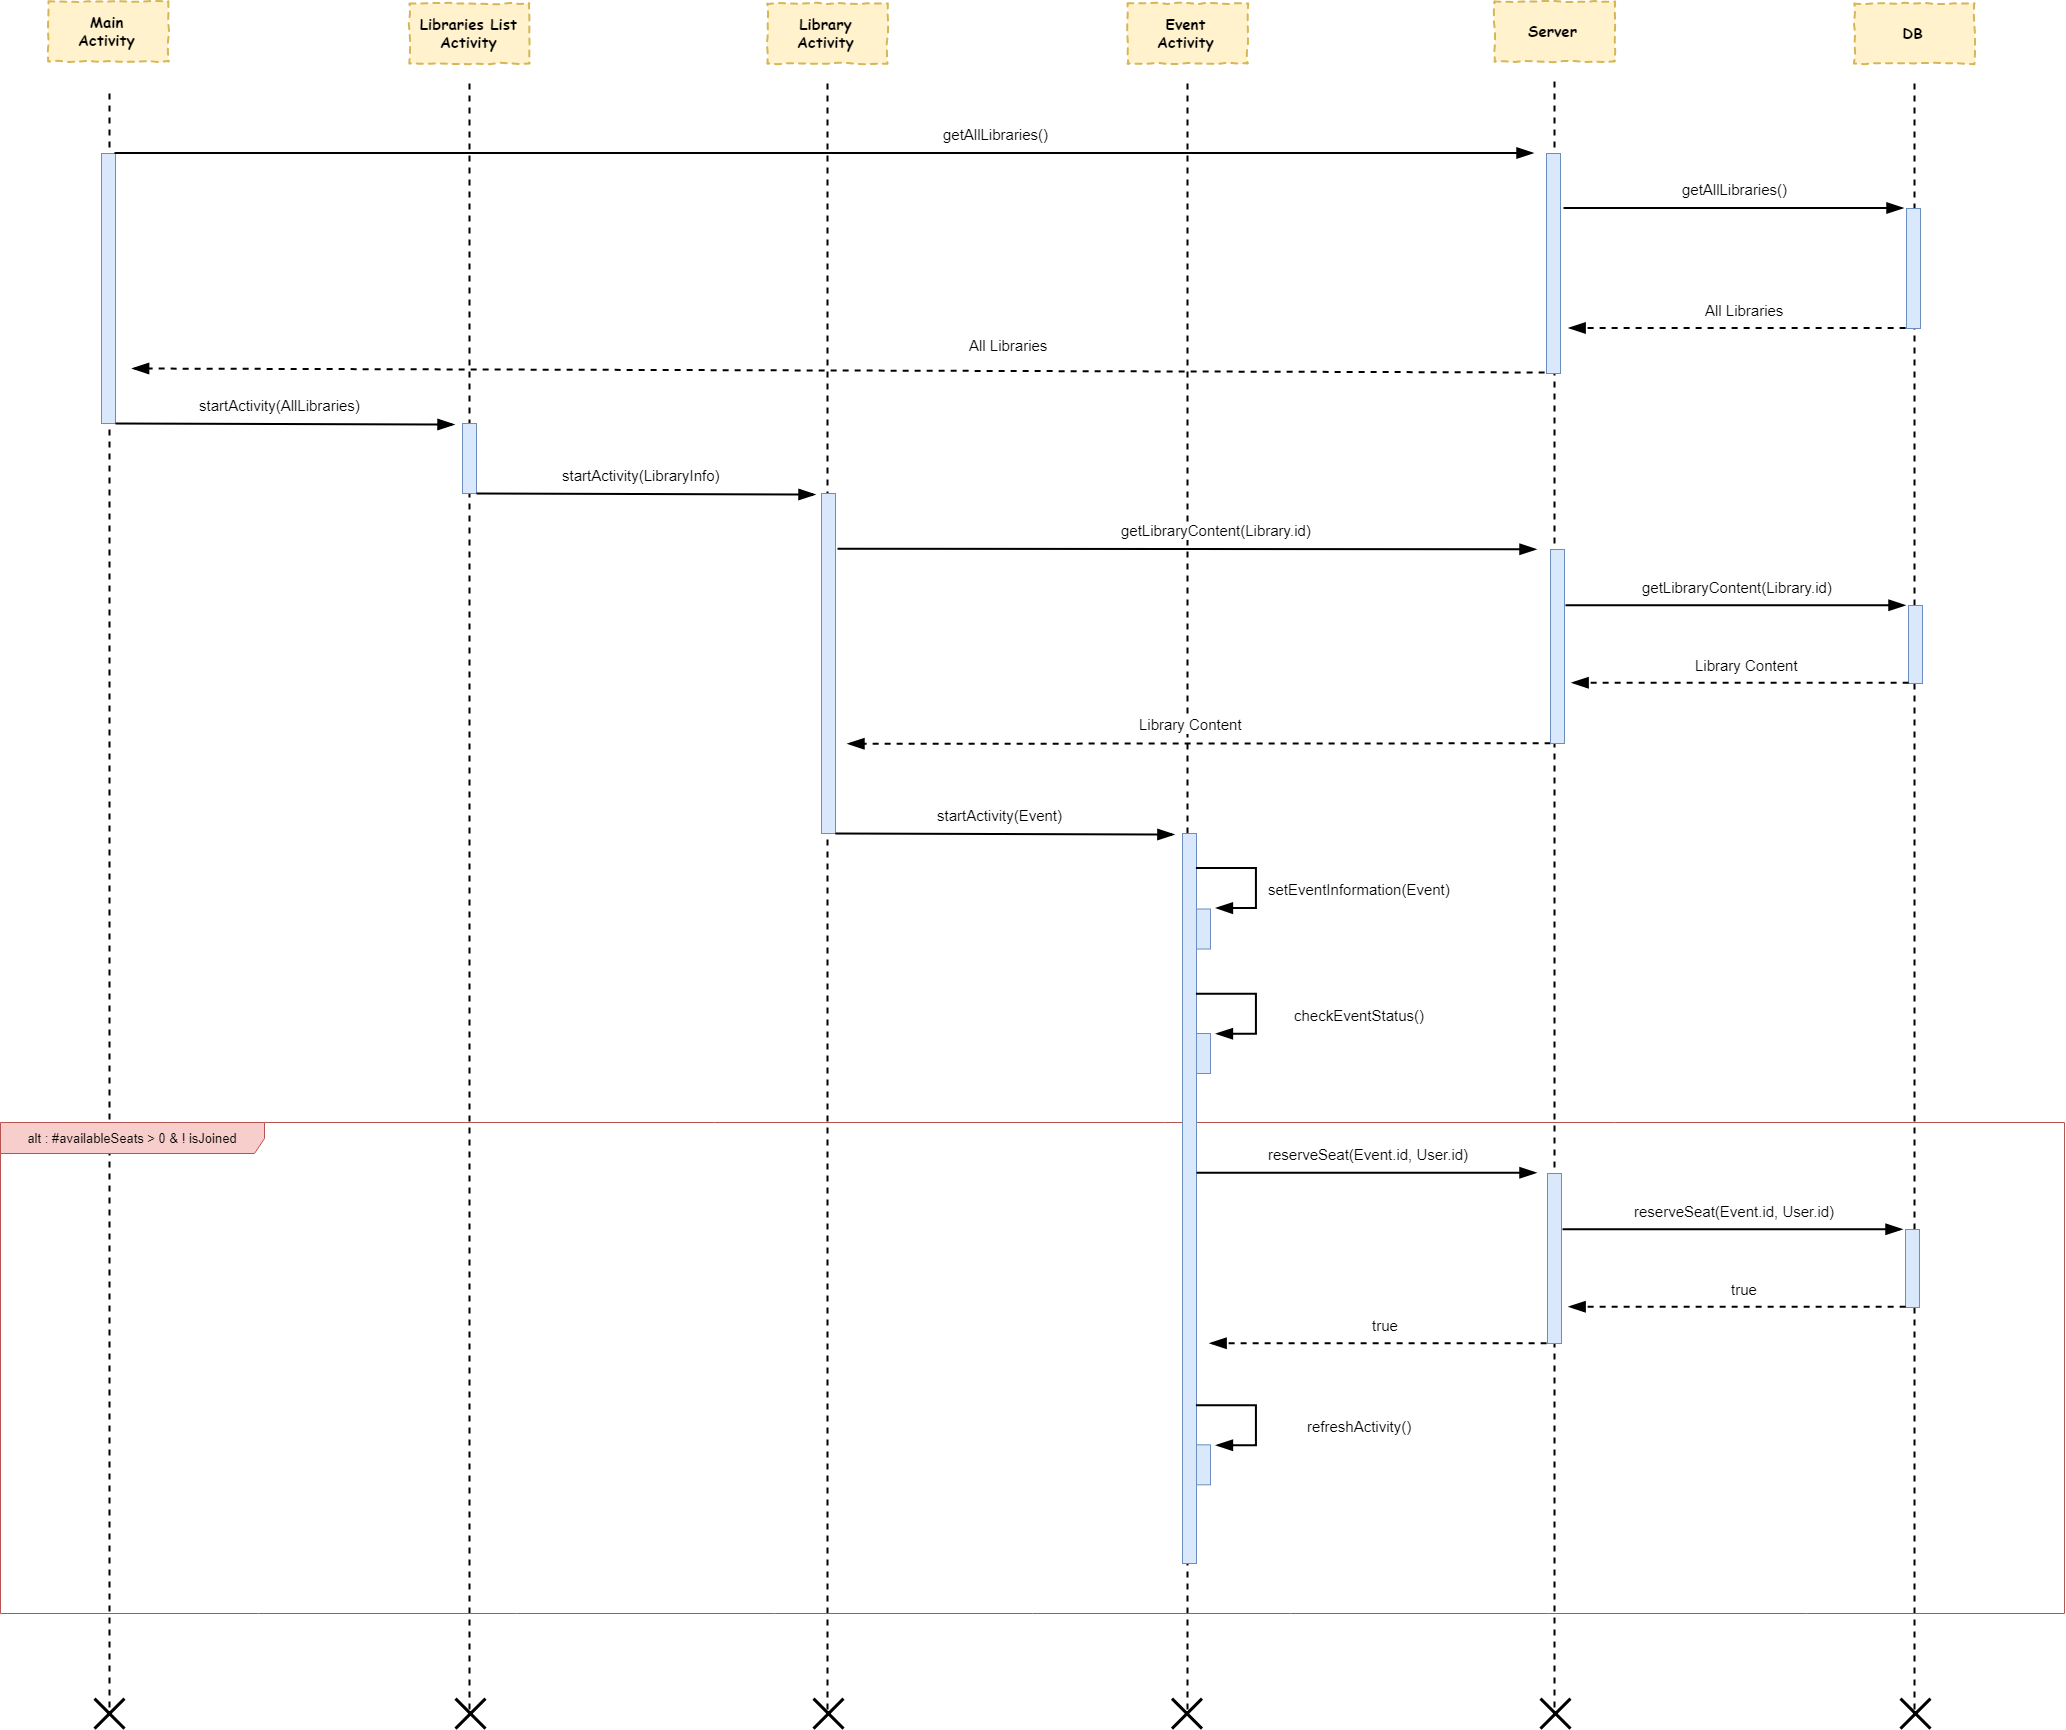
\includegraphics[scale=0.22]{Images/Runtime/event_reserve_seat}
	\caption{Event Reserve Seat - Runtime View}
\end{figure}

\newpage
\vspace*{0cm}
\mysubsection{EasyLib - Librarian}
\vspace*{0.5cm}

\mysubsubsection{QR-Code Scan + Book Returned}
This Runtime View shows the different steps needed to find book information through QR-code scan and communicate to the serve (and so the DB) that the book is returned.\par
We have to make an assumption : in the following diagram we reported only the most meaningful calls needed to achieve the goal.\par
So starting from the "Library Activity" the librarian has to tap the Floating Button with the QR-code icon that allows the app to open the "QR Scan Activity". As in the previous runtime, the qr-code is analyzed and the identifier returned is used to get from the server (and so the DB) the information of that specific book. The "Book Activity" is then opened and data are set in the layout.\par
The app has next to get all the reservations and pass the ArrayList to an Adapter that generates the single items of the recyclerView placed under the book layout.\par
At the end the librarian as to find the reservation that has the user id and tap the "Returned" button.
\newpage
\vspace*{0cm}
\begin{figure}[H]
	\centering
	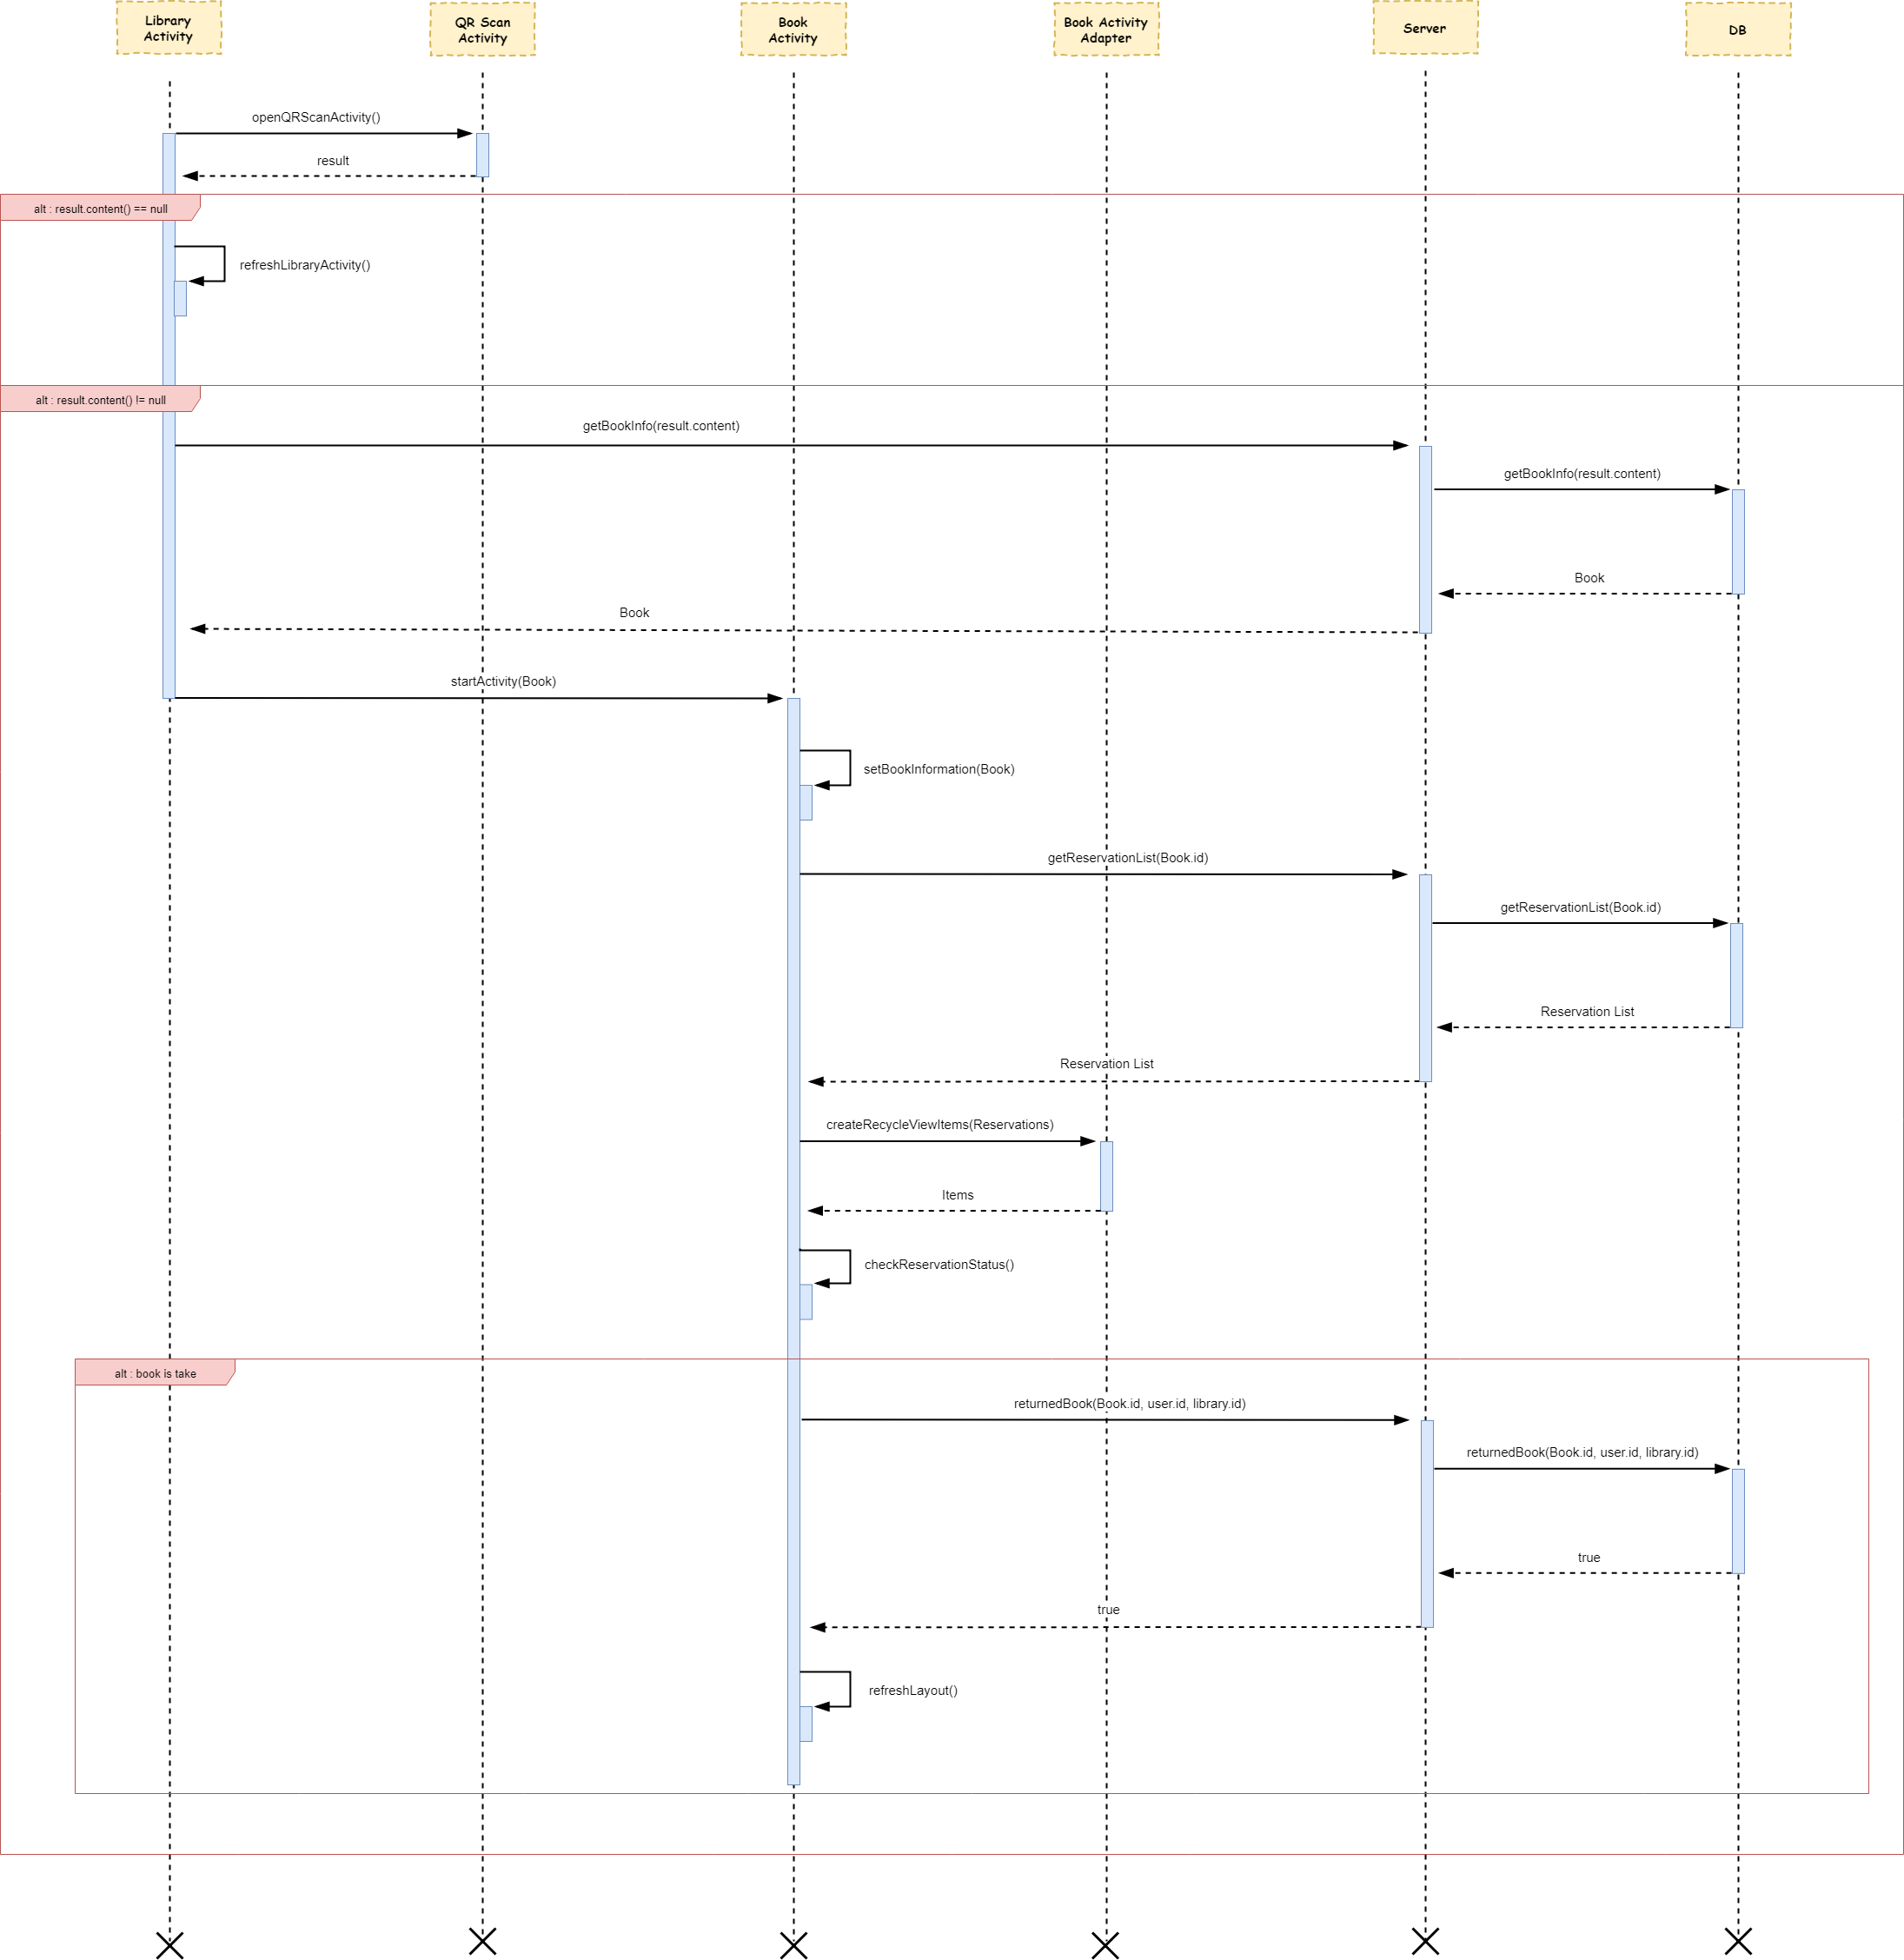
\includegraphics[scale=0.21]{Images/Runtime/librarian_qrcode_returned}
	\caption{QR-Code Scan + Book Returned - Runtime View}
\end{figure}